\section{규칙파 검증 실험 및 결과}

\subsection{조파기 구동 코드}

\begin{algorithm}[h]
    \caption{Sinusoidal Motion}
    \label{Sinusoidal Motion}
    \begin{algorithmic}[1]
    \Procedure{Sinusoidal Motion}{$A, N, \Delta\phi$}\Comment{Move the motor by sinusoidal function}
        \For{$elapsed Time \geq 0$}
            \If{$elapsed Time \geq N$}
                \State {$elapsed Time$ = 0}
                \State {$target = f(n)$}%\Comment{In this case, $target$ = $A \sin${($n$ $\Delta$$\phi$)}}
                % \State {$target$ = $A \sin${($n$ $\Delta$$\phi$)}}
                \State {$n$ $\gets$ $n$ + 1}
                \State {Move $motor$ to $target$}
            \EndIf
        \EndFor
        \EndProcedure
    \end{algorithmic}
\end{algorithm}

조파기 구동 코드는 시간간격 $N$마다 ($N$은 $\mathrm{~ms}$ 단위이다) 각 변위를 $f(n)$으로 지정하는 방식으로 작동한다 (알고리즘 \ref{Sinusoidal Motion}). 이 함수가 $\sin$형이면 모터가 사인형 각 변위를 따라 움직일 것으로 기대할 수 있다. sin형 구동을 위한 코드의 $f(n)$은 다음과 같다.
\begin{equation}
    f(n) = A \sin(n \Delta\phi)
    \label{f(n)}
\end{equation}

하지만 실질적인 매개변수는 $A, \omega, N$이며 $A$는 진폭, $\omega$는 조파판 위상의 각진동수, $N$은 조파판의 변위를 업데이트하는 시간 간격이다. $\omega$는 다음과 같이 정의될 수 있다.

\begin{equation}
    \omega = \frac{\Delta\phi}{\Delta t} = \frac{\Delta\phi}{N}, ~\Delta\phi = N \omega
    \label{f(N)}
\end{equation}

즉, $N$과 $\omega$가 매개된 입력 신호의 식을 알 수 있다. $A$와 $\omega$는 코드에서의 입력값과 조파기 구동 시 판의 움직임에서 실제로 나타나는 값이 달라 그 관계를 파악하기 위한 실험이 필수적이며, $\omega$를 크게 할 경우 탈조가 날 수 있어 가능 범위를 파악해야 한다. $N$은 이론적으로 조파판의 움직임에 영향을 주는 요소가 아니어서 이를 고정하여 실험을 진행했으나, 판의 최대 변위와 최소 변위 지점에서 변위가 업데이트되어야 하므로 각진동수에 따른 $N$의 변화가 필요할 수 있다. 즉, 각진동수의 크기에 따라서 최선의 $N$이 있을 수 있다는 것이다.

\subsection{예비 실험}
$A$는 $5\mathrm{~cm}$, $N$은 50으로 고정한 후, $\omega$를 $0.4\pi$에서 $\pi$까지 $0.1\pi$ 간격으로 변화시키며 실험하고 추가로 $1.5\pi$에 대해 실험을 진행하였다. 
이 경우 판의 움직임을 분석했을 때 $\omega$가 증가함에 따라 진폭의 출력값이 감소하는 것을 확인할 수 있었다. 생성되는 파의 경우, sin파 형태와 유사하고 각진동수는 입력값과 동일했지만 진폭은 관계가 없어서 실험 구성 단계에서는 모터의 움직임만 분석하기로 결정하였다. 

\subsection{실험 구성}
생성파의 분석이 필요치 않으므로 조파기의 모터 대신 작은 모터에 회로를 연결하여 모터의 움직임이 sin 형태인지를 확인하였다. 이는 시리얼 모니터에 현재 각 위치를 출력하여 알 수 있다. 각진동수의 출력값은 입력값과 일치하나 진폭은 달랐으며, $\omega$가 클수록 진폭의 출력값이 감소하였다 (그림 \ref{PreExperiment}).

\begin{figure}[H]
    \centering
    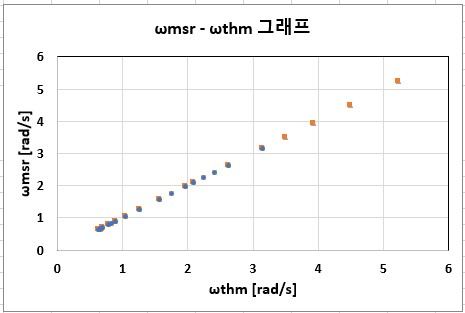
\includegraphics[height=5cm]{images/PreExperiment_Graph(Omega-Omega)-junlam.jpg}
    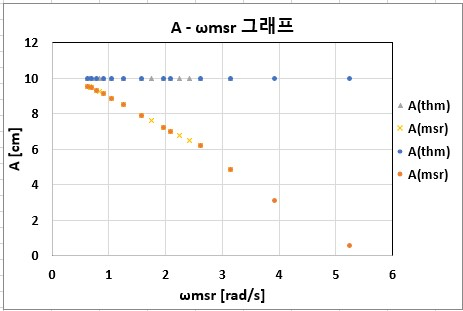
\includegraphics[height=5cm]{images/PreExperiment_Graph(A-Omega)-junlam.jpg}
    \caption{$\omega_{msr}$(측정값)에 대한 $\omega_{thm}$(입력값) (좌),  $\omega_{msr}$에 대한 진폭 $A_{msr}$(측정값) (우) - 예비 실험}
    \label{PreExperiment}
\end{figure}

그러므로 우리가 파를 생성하려고 할 때 구동 코드의 매개변수에 따른 판의 움직임과 생성되는 파 2개를 관찰해야 한다. 그리고 두 파의 진폭과 각진동수를 코드의 값과 비교하여 관계를 파악하는 것을 목표로 한다.

\begin{figure}[H]
    \centering
    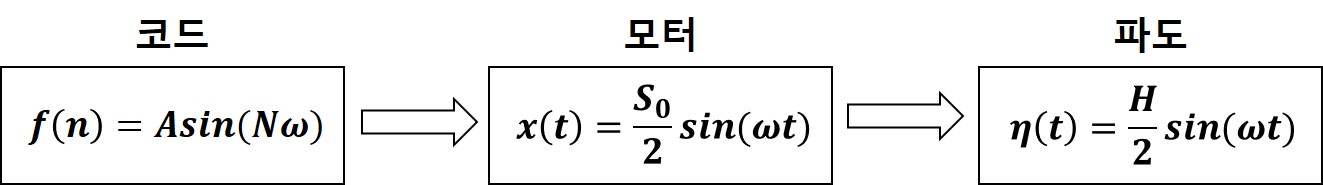
\includegraphics[width=12cm]{images/Flow_Chart(Analysis System_Kor).jpg}
    \caption{조파기 검증 실험의 흐름도}
    \label{Flow_Chart}
\end{figure}

비록 $S_0$와 $A$의 관계는 알 수 없으나 $S_0$와 $H$의 관계는 이론적 배경의 식을 따를 것으로 기대할 수 있으며 파가 sin형이 아니더라도 FFT 분석을 통해서 $\omega$를 구할 경우 세 파동에서 일관될 것이라고 예측할 수 있다.
이를 제대로 검증하기 위해서는 다양한 조건에 대한 데이터가 필요하며 이론적 분석과 예비 실험을 통해 정한 범위는 $A$는 $1\mathrm{~cm}$부터 $10\mathrm{~cm}$까지 $1\mathrm{~cm}$ 간격으로, $\omega$는 $3$부터 $12$까지 $1$ 간격으로 변화시키는 것이다. $N$은 50으로 고정시켰다 (단, 수심은 $15\mathrm{cm}$로 고정하였다).

%실험한 내용을 집어넣어야 함.

%실험계의 모식도가 필요함. 혹은 사진이라도.
\subsection{성능 검증 실험 결과}

\begin{figure}[H]
    \centering
    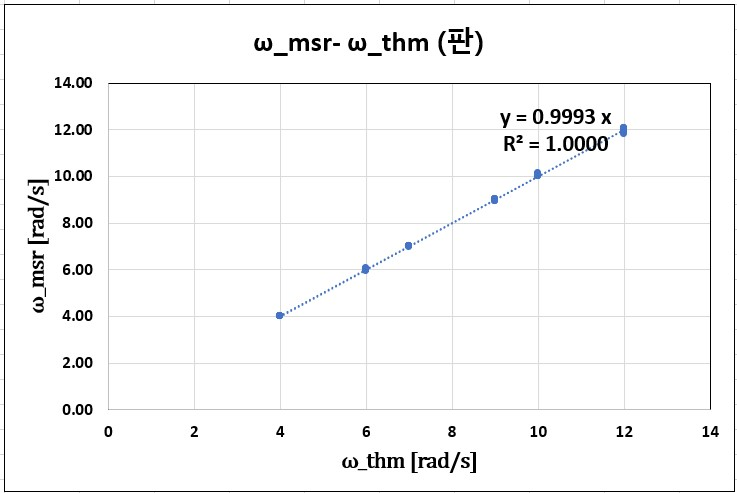
\includegraphics[height=5cm]{images/Experiment(omega_thm-omega_msr)_Plate_Kor.jpg}
    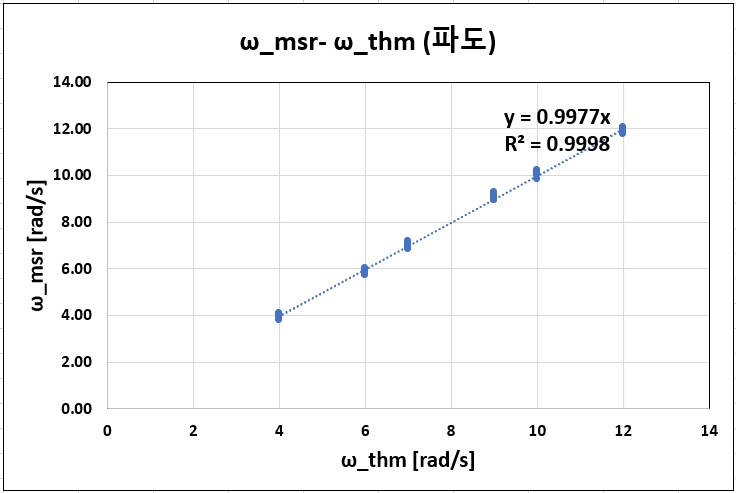
\includegraphics[height=5cm]{images/Experiment(omega_thm-omega_msr)_Wave_Kor.jpg}
    \caption{측정한 $\omega_{msr}$에 대한 코드의 $\omega_{thm}$ (좌),  $\omega_{msr}$에 대한 측정 진폭 $A_{msr}$ (우) - 검증 실험}
    \label{ExperimentGraph - 1, 2}
\end{figure}

그림 \ref{ExperimentGraph - 1, 2}에서 알 수 있듯이 $\omega$는 코드에서 대입한 값과 판, 파도 모두 같은 값을 띔을 알 수 있다 (두 그래프 모두 선형 관계를 만족하며($R^2 > 0.99$) 그 기울기는 약 1.000이다). 또, 분산 관계식과 식 \ref{eq:5}을 통해 주어진 $\omega$에 대한 $H/S$를 예측할 수 있고 이를 측정값과 비교해보았다 (그림 \ref{H/S Graph}).

\begin{figure}[H]
    \centering
    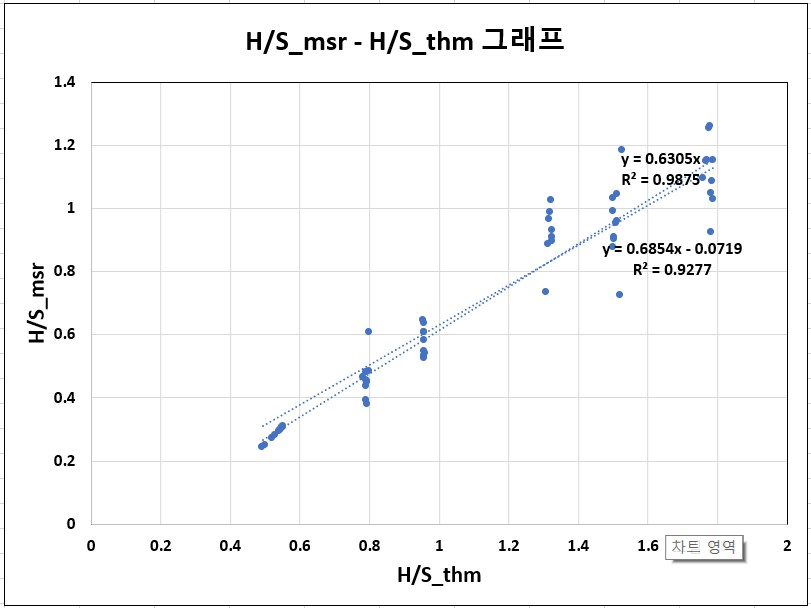
\includegraphics[width=0.70\textwidth]{images/Experiment(H.S_thm-H.S_msr).jpg}
    \caption{$H/S_{msr} - H/S_{thm}$ 그래프}
    \label{H/S Graph}
\end{figure}

$H/S$는 선형 관계를 만족한다고 볼 수 있다. 측정값이 구간으로 나타났으나 이는 불확도 내의 값으로 취급할 수 있으며 선형 추세선의 기울기가 $1.000$은 아니지만 선형 추세를 통해 매개변수로부터 $H/S$를 예측할 수 있다.

\begin{figure}[H]
    \centering
    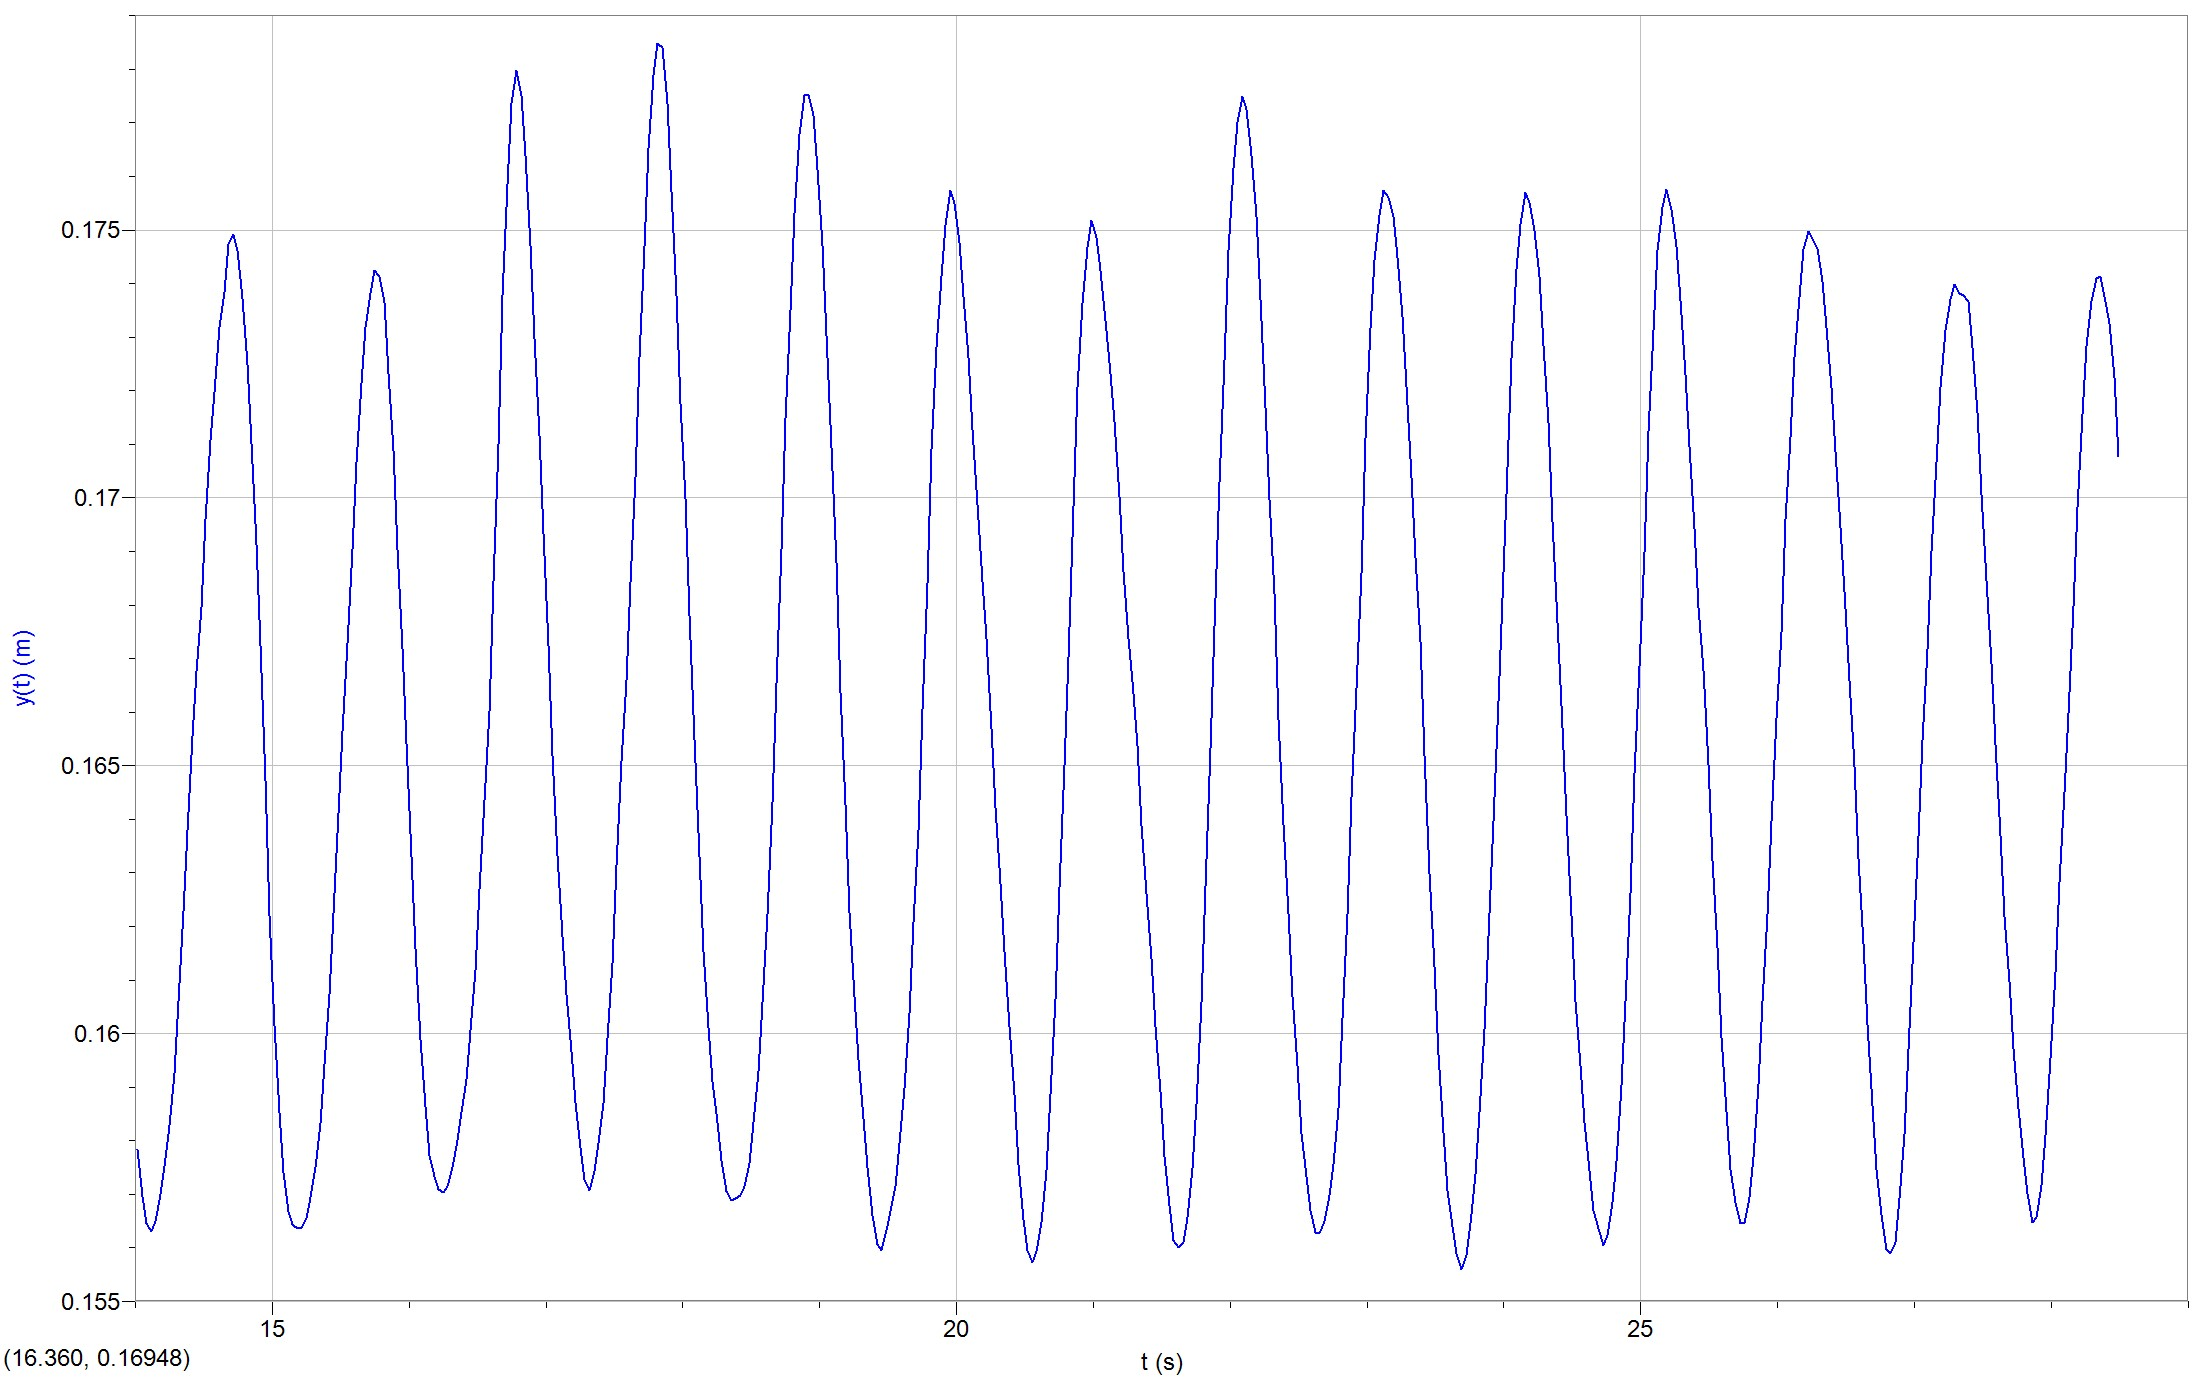
\includegraphics[width=0.70\textwidth]{images/Wave(omega=6,A=2).jpg}
    \caption{파형 데이터($A=2\mathrm{cm},~\omega=6\mathrm{rad/s}$)}
    \label{Example Wave Data}
\end{figure}

그림 \ref{Example Wave Data}는 한 sin 파의 예시이다. 코드에서는 $A=2\mathrm{cm},~\omega=6\mathrm{rad/s}$를 대입하였으며 측정값은 $A=0.9588\mathrm{cm},~\omega=5.959\mathrm{rad/s}$이다. 

\subsection{오차 원인}

본 실험에서는 실험 과정에서의 오차, 분석 상의 오차 등 여러 오차가 존재한다. 이는 크게 모터에 의한 것과 파고계 영상 분석에 의한 것으로 나눌 수 있다.

모터의 한계에 의한 것은 $\omega$에 따른 A의 한계와 아두이노에서 업로드한 파의 형태에 오차가 생기는 것이다. 최대 각가속도가 판 움직임의 진폭과 오차를 결정한다는 것은 실험을 통해 알 수 있었다. 실험은 $\omega = 6$, A = 5cm로 설정한 상태로, 각가속도만 $30,000\mathrm{step/s^2}, 40,000\mathrm{step/s^2}, 50,000\mathrm{step/s^2}$로 바꿔가며 판의 움직임을 조사하는 것으로 진행하였다. 이 때 판 움직임을 위상이 같도록 정렬한 결과가 아래의 그림이다. x축은 시간이고 y축은 판의 변위$(\mathrm{m})$이고 눈금 한 개의 스케일은 $0.01\mathrm{m}$이다.

\begin{figure}[H]
    \centering
    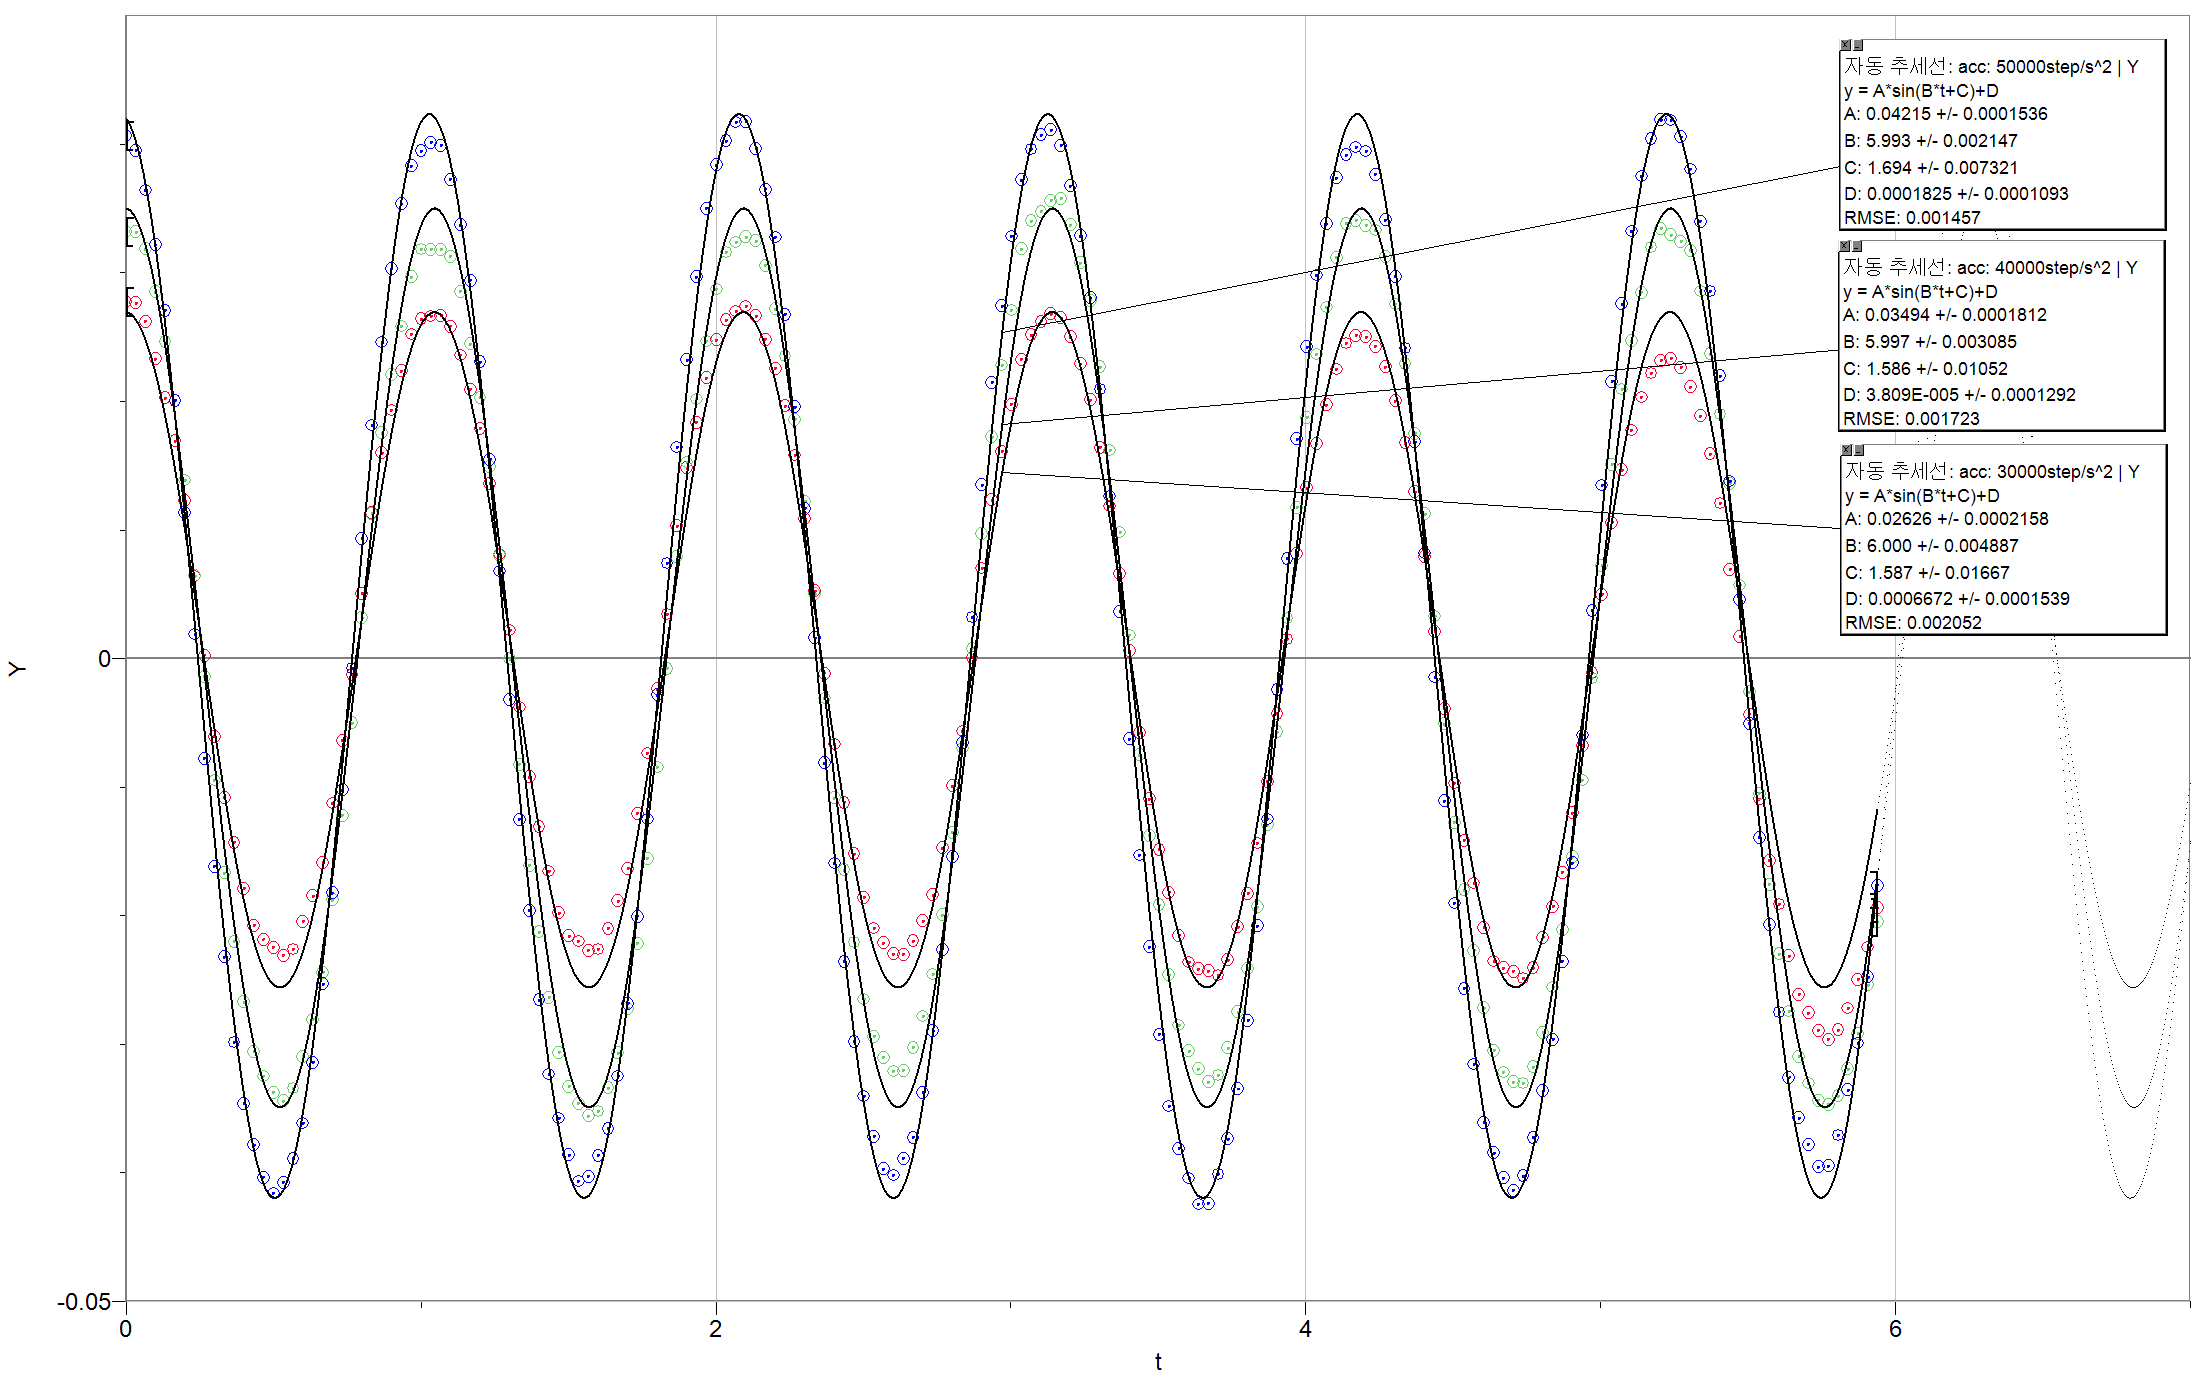
\includegraphics[width = 15cm, height = 10cm]{images/singraphofdiffacc.png}
    \caption{각가속도를 다르게 한 경우의 파고 데이터}
    \label{fig:enter-label}
\end{figure}
결과를 정리하면 각각은 다음과 같은 진폭과 진동수를 가진다.


\begin{table}[H]
    \centering
    \begin{tabular}{l|ll}
    \hline
    각가속도$(\mathrm{step/s^{2}})$ & $A (\mathrm{m})$ & RMSE \\
    \hline
    30,000 & 0.02626 & $2.052\times10^{-3}$ \\
    40,000 & 0.03494 & $1.723\times10^{-3}$ \\
    50,000 & 0.04215 & $1.457\times10^{-3}$\\
    \hline
    \end{tabular}%
\end{table}

해석하자면 목표한 진폭인 $5\mathrm{cm}$에 도달하지 못한 이유는 파의 구현에 필요한 각가속도가 $50,000\mathrm{step/s^2}$보다 크기 때문이라 볼 수 있는데, 물의 높이 $15\mathrm{cm}$를 기준으로 파가 중첩되어 생길 수 있는 최대 물의 높이에서 모터가 탈조나지 않기 위한 조건이 각가속도가 $30,000\mathrm{step/s^2}$ 이하일 것이기에 사용 중인 스텝모터로는 위의 $A-\omega$ 그래프에서 확인할 수 있는 정상적으로 구현되는 파만 구현 가능하다는 결론이 나온다.

%파도의 높낮이 변화가 극단적인 경우 부표식 파고계의 스티로폼 조각이 물 속에 잠겨버림->그로 인해서 진폭이 이론값보다 작게 나타남

%팽팽하게 위로 늘어났다가 풀리며 작은 마루가 옆에 생겨나는 현상도 관찰됨'

%쇄파 현상으로 인해 부표 위의 표식을 트래킹할 수 없

또, 본 실험에서는 스펀지와 유사한 재질의 포장재를 이용하여 얇은 직사각형판 모양의 부표를 만들었다. 이의 위치를 트래킹하여 파고를 측정하는데, 부표의 재질이 스펀지와 비슷하게 구멍이 많이 뚫려있는 재질이기에 파도의 높낮이 변화가 극단적일 경우, 물 위에 뜨지 못하고 잠시 잠기는 현상이 나타난다. 이로 인해 진폭이 이론값보다 작게 측정되는 오차가 있다. 또한 부표가 y축을 따라서만 움직이고 파도의 진행 방향에 영향을 받지 않도록 하기 위하여 부표에 두 개의 구멍을 뚫어 실을 통과시킨 후 이를 따라 움직이도록 하였는데, 마찰이 존재하므로 부표가 파도를 따라 위로 올라가는 과정에서 실이 늘어나게 된다. 실의 탄성에 의해 내려오는 과정에서 위로 튕기게 되어 파도의 큰 마루 옆에 작은 마루가 생기는 오차가 발생한다. 마지막으로, 쇄파 현상이 생기는 경우, 부표의 정중앙 표식이 부서지는 파도에 의해 가려져 정확히 같은 지점을 트래킹하는 것이 불가능하다.

%다 쓰면은 쌤한테 끝났다고 얘기하면 됨. 알겠냐?